
% Лабораторная работа по криптографии № 1
% Михедов Константин Константинович

% Тип документа: статья, на бумаге А4
\documentclass[a4paper]{article}

% Подключение сторонних tex файлов 
\usepackage{import}


% Основные данные - ВУЗ, факультет, город...
\import{./../../stuff/tex}{config.tex}
% Небольшой набор инструментов
\import{./../../stuff/tex}{tools.tex}

% Подключение необходимых зависимостей
\import{./../../stuff/tex/settings}{packages.tex}
% Настройка подключенных пакетов
\import{./../../stuff/tex/settings}{preferences.tex}


% Шаблон титульной страницы 
\import{./../../stuff/tex/templates}{title.tex}
% Упрощенный блок "выполнил"
\import{./../../stuff/tex/templates}{sign2.tex}
% Макрос для содержания
\import{./../../stuff/tex/templates}{toc.tex}

% Определяем название документа
\title{
  ОТЧЕТ \\
  О ПРАКТИЧЕСКОЙ РАБОТЕ №2 \\
  по дисциплине <<Основы криптографии и стеганографии>> \\
  БЛОЧНЫЕ ШИФРЫ  
}
% Указываем преподавателя
\renewcommand{\teachername}{
    Заведующий кафедрой информационной безопасности киберфизических систем \\
    канд. техн. наук, доцент \\
    \entryline{3.5cm} О.О. Евсютин
}


% Путь до внешних изображений
\graphicspath{ {./figures/}}
% Нумеруем все формулы
\mathtoolsset{showonlyrefs=false}


% Основной текст работы
\begin{document}
  \templatedtitlepage
  
  \toc

  \section{Здание на практическую работу}

  Целью данной практической работы является программная реализация и последующий 
  криптоанализ некоторых блочных шифров.

  В рамках работы необходимо выполнить следующие шаги:

  \begin{enumerate}
    \setlength{\itemindent}{1cm}
    \item {
        Программно реализовать следующие подстановочные шифры 

        \begin{itemize}
            \setlength{\itemindent}{1cm}
            \item Шифр Хилла
            \item Рекуррентный шифр Хилла
        \end{itemize}
    }
    \item {
        Изучить и описать методы криптографического анализа данных шифров 
    }
    \item {
        Провести криптоанализ данных шифров
    }
    \item {
        Подготовить отчет о проделанной работе
    }
  \end{enumerate}

  \newpage
  \section{Краткая теоретическая часть}

  \subsection{Описание шифров}

  \subsubsection{Шифр Хилла}

  Допустим, имеется сообщение $X$ длиной $n$ символов: $X = (x_1, x_2, \dots, x_n)$,
  где $x_i$ - $i$-ый символ данного сообщения, пренадлежит алфавиту $A$ мощности $m$.

  Для получения шифртекста необходимо задать ключ - невырожденную (определитель не равен нулю)
  матрицу K размером $t \times t$ вида (\ref{eq:key_h}), причем НОД$(|K|, m)$ должен быть 1.
  \begin{equation}
    K = \begin{pmatrix}
        k_{11} & k_{12} & \dots & k_{1t} \\
        k_{21} & k_{22} & \dots & k_{2t} \\
        \vdots & \vdots & \ddots & \vdots \\
        k_{t1} & k_{t2} & \dots & k_{tt} \\
    \end{pmatrix}
    \label{eq:key_h}
  \end{equation}

  Далее исходный текст делится на блоки по $t$ символов (блоки с недостаточным количеством символов
  дозаполняются до необходимой длины какими угодно символами), тогда для каждого блока (вида $B = (b_1, b_2, \dots, b_t)$)
  определяются операции зашифровки (\ref{eq:en_h}) и расшифровки (\ref{eq:deq_h}):
  \begin{equation}
    E_K(B) = E_K(b_1, b_2, \dots, b_t) = \underset{\text{матричное умножение}}{\underbrace{K \cdot \begin{pmatrix}
        b_1, b_2, \dots, b_t
    \end{pmatrix}}} = \begin{pmatrix}
        c_1, c_2, \dots, c_t
    \end{pmatrix}
    \label{eq:en_h}
  \end{equation}
  \begin{equation}
    D_K(C) = D_K(c_1, c_2, \dots, c_t) = \underset{\text{матричное умножение}}{\underbrace{K^{-1} \cdot 
    \begin{pmatrix}
        c_1, c_2, \dots, c_t
    \end{pmatrix}
    }} = \begin{pmatrix}
        b_1, b_2, \dots, b_t
    \end{pmatrix}
    \label{eq:deq_h}
  \end{equation}

  Для зашифрования целого текста поочередно шифруется каждый блок, позже результаты просто объединяются в один в необходимом порядке.

  \subsubsection{Рекуррентный шифр Хилла}

  Для данного шифра также потребуется исходное сообщение $X_n$ и алфавит $A_m$, а также
  целых два ключа - $K_1$ и $K_2$, каждый из которых - матрица размером $t \times t$ такая, что ее определитель
  взаимно простой с мощностю алфавита.

  Далее исходный текст снова делится на блоки по $t$ симовлов: $X_n \rightarrow B_1, B_2, \dots, B_3$,
  шифрование каждого блока выполняется по формуле (\ref{eq:en_h}): $C_i = E_{K_i}(B_i)$, причем
  $K_1$ и $K_2$ заданы изначально, а все последующие вычисляются по формуле (\ref{eq:key_rh}):
  \begin{equation}
    K_i = K_{i - 2} \cdot K_{i - 1}
    \label{eq:key_rh}
  \end{equation}

  Расшифрование выполняется аналогично: $B_i = D_{K_i}(C_i)$. Полученные блоки склеиваются в исходной последовательности, благодаря чему получается шифртекст или открытый текст.

  \subsection{Методы криптографического анализа}

  \subsubsection{Метод грубой силы}

  Метод заключается в полном переборе всех возможных ключей до тех пор, пока не будет найден подходящий
  для корректного расшифрования. Его сложность зависит от многих факторов: размер ключа, мощность алфавита
  и тп.

  Так как все операции в зашифровании и расшифровании происходят по подулю мощности алфавита,
  то каждый элемент ключа может принимать целочисленные значения в полуинтервале $[0; m)$.
  Таким образом, чтобы подобрать ключевую матрицу размером $2 \times 2$ потребуется в
  худшем случае перебрать $m^{2 * 2} = m^4$ вариантов различных ключей.

  Если взять алфавит большой мощности или достаточно большой ключ, то сложность полного
  перебора будет весьма значительной, что сделает данный метод абсолютно нерелевантным.
  Так же стоит учитывать тот факт, что может быть неизвестен размер исходного ключа,
  что вынудит злоумышленника перебирать все возможные размеры, что опять таки увеличит
  сложность, время и ресурсозатратность метода грубой силы.

  Для рекуррентного шифра Хилла сложность полного перебора квадратично возрастает, что делает
  данных шифр еще более стойким к методу грубой силы.

  \subsubsection{Частотный анализ}

  Обычный шифр Хилла легко подвергается частотному анализу при размере ключа, равном 1,
  так как фактически становится Афинным шифром. Однако опасность частотного анализа
  не исчезает и при больших размерах ключа.

  Да, станет невозможно сопоставить частотность встречания отдельных букв, однако биграммы и триграммы
  сохраняться, что позволит посторить соответсвия, благодаря которым можно будет взломать шифр.

  Рекуррентный шифр Хилла не создает таких точных биекций (так как на каждый блок открытого текста
  ключевая матрица потенциально уникальна), что делает его устойчивым к атакам на основе частотного анализа.

  \subsubsection{Атаки на основе открытого текста}

  Если в руки злоумышленника попала какая-то часть открытого текста, он может попытаться с ее
  помощью найти использованный для зашифрования ключ.

  Для взлома обычного шифра Хилла злоумышленнику необходимо найти соответствие между $n$ любыми блоками
  открытого текста и шифртекста, где $n$ - длина блока для шифрования или расшифрования. Тогда
  будет необходимо всего лишь решить систему из нескольких уравнений, после чего ключ будет найден.

  При больших размерах ключа или система уравнений может стать весьма сложной, или злоумышленнику потребуется найти
  достаточно большой кусок открытого текста для выполнения расшифрования.

  В случае рекуррентного шифра Хилла все несколько сложнее. Во-первых, для того, чтобы была возможность
  составить систему уравнений для поиска ключа необходимо найти соответсвие между $n$ \textbf{подрядыдущими}
  блоками открытого и шифртекста. Во-вторых, полученная система окажется гораздо более сложной.

  Однако оба шифра уязвимы к атакам подобного вида.

  \newpage
  \section{Примеры ручного шифрования}

  В качестве алфавита будет использоваться английкий, состоящий только из маленьких букв. Его мощность составляет 26 символов.

  Также установим, что нумерация букв в алфавите начинается с 0

  \subsection{Шифр Хилла}

  Для первого примера зашифруем слово <<abobus>> с помощью следующего ключа (\ref{eq:k1}):
  \begin{equation}
    K = \begin{pmatrix}
        1 & 3 \\ 2 & 3
    \end{pmatrix}
    \label{eq:k1}
  \end{equation}

  Заметим, что $\det{K} = 1\cdot 3 - 2\cdot 3 = -3$, что не является нулем, а также взаимнопростое
  с мощностью алфавита, то есть с 26.

  Сопоставим каждой букве ее порядковый номер, так <<abobus>> $ = (0, 1, 14, 1, 20, 18)$.
  Данный открытый текст разобъется на три блока: $B_1 = (0, 1)$, $B_2 = (14, 1)$, $B_3 = (20, 18)$.
  Выполним зашифрование каждого блока по очереди:
  \begin{equation} C_1 = K\cdot B_1 =
    \begin{pmatrix}
        1 & 3 \\ 2 & 3
    \end{pmatrix} \cdot \begin{pmatrix}
        0 \\ 1
    \end{pmatrix} = \begin{pmatrix}
        0\cdot 1 + 3\cdot 1 \\ 0 \cdot 2 + 1 \cdot 3
    \end{pmatrix} = \begin{pmatrix}
        3 \\ 3
    \end{pmatrix} \Leftrightarrow \begin{pmatrix}
        d \\ d
    \end{pmatrix}
  \end{equation}
  \begin{equation}
    C_2 = K\cdot B_2 = 
    \begin{pmatrix}
        1 & 3 \\ 2 & 3
    \end{pmatrix} \cdot \begin{pmatrix}
        14 \\ 1
    \end{pmatrix} = \begin{pmatrix}
        14 + 3 \\ 28 + 3
    \end{pmatrix} = \begin{pmatrix}
        17 \\ 31
    \end{pmatrix} \Leftrightarrow \begin{pmatrix}
        r \\ f
    \end{pmatrix}
  \end{equation}
  \begin{equation}
    C_3 = K\cdot B_3 = \begin{pmatrix}
        1 & 3 \\ 2 & 3
    \end{pmatrix} \cdot \begin{pmatrix}
        20 & 18
    \end{pmatrix} = \begin{pmatrix}
        20 + 54 \\ 40 + 54
    \end{pmatrix} = \begin{pmatrix}
        74 \\ 94
    \end{pmatrix} \Leftrightarrow \begin{pmatrix}
        w \\ q
    \end{pmatrix}
  \end{equation}

  Объединяем полученные блоки воедино и получаем, что $E_K(\text{<<abobus>>}) = \text{<<ddrfwq>>}$

  Для расшифрования потребуется найти обратимую для ключа матрицу, то есть такую матрицу $K^{-1}$,
  что $K\cdot K^{-1} \mod{m} = E$, где $E$ - нулевая матрица с единицами на главной диагонали.
  \begin{equation}
    \begin{pmatrix}
        1 & 3 \\ 2 & 3
    \end{pmatrix} \cdot \begin{pmatrix}
        25 & 1 \\ 18 & 17
    \end{pmatrix} \mod{26} = \begin{pmatrix}
        1 & 0 \\ 0 & 1
    \end{pmatrix} \Rightarrow K^{-1} = \begin{pmatrix}
        25 & 1 \\ 18 & 17
    \end{pmatrix}
  \end{equation}

  Произведем расшифрование с помощью полученного $K^{-1}$:
  \begin{equation}
    B_1 = K^{-1}\cdot C_1 = \begin{pmatrix}
        25 & 1 \\ 18 & 17
    \end{pmatrix} \cdot \begin{pmatrix}
        3 \\ 3
    \end{pmatrix} = \begin{pmatrix}
        78 \\ 105
    \end{pmatrix} \Leftrightarrow \begin{pmatrix}
        a \\ b
    \end{pmatrix}
  \end{equation}
  \begin{equation}
    B_2 = K^{-1}\cdot C_2 = \begin{pmatrix}
        25 & 1 \\ 18 & 17
    \end{pmatrix} \cdot \begin{pmatrix}
        17 \\ 31
    \end{pmatrix} = \begin{pmatrix}
        456 \\ 833
    \end{pmatrix} \Leftrightarrow \begin{pmatrix}
        o \\ b
    \end{pmatrix} 
  \end{equation}
  \begin{equation}
    B_3 = K^{-1}\cdot C_3 = \begin{pmatrix}
        25 & 1 \\ 18 & 17
    \end{pmatrix} \cdot \begin{pmatrix}
        74 \\ 94
    \end{pmatrix} = \begin{pmatrix}
        1944 \\ 2930
    \end{pmatrix} \Leftrightarrow \begin{pmatrix}
        u \\ s
    \end{pmatrix} 
  \end{equation}

  Видно, что расшифровка дала верный результат.

  \subsection{Рекуррентный шифр Хилла}

  Зашифруем слово <<cringe>>, соответствующее следующей числовой последовательности
  $(2, 17, 8, 13, 6, 4)$, при помощи ключей:
  \begin{align}
    K_1 = \begin{pmatrix}
        1 & 3 \\ 2 & 3
    \end{pmatrix} &&  K_2 = \begin{pmatrix}
        1 & 2 \\ 3 & 1
    \end{pmatrix}
  \end{align}

  Заметим, что $\det{K_1} = -3$, а $\det{K_2} = 1\cdot 1 - 2\cdot 3 = -5$. Оба числа не равны
  нулю и взаимнопросты с 26 (мощностью алфавита).

  Исходный текст поделится на 3 блока, поэтому потребуется вычислить $K_3$:
  \begin{equation}
    K_3 = K_1\cdot K_2 = \begin{pmatrix}
        1 & 3 \\ 2 & 3
    \end{pmatrix} \cdot \begin{pmatrix}
        1 & 2 \\ 3 & 1
    \end{pmatrix} = \begin{pmatrix}
        10 & 5 \\ 11 & 7
    \end{pmatrix}
  \end{equation}

  Разобъем открытый текст на блоки $B \rightarrow$ $B_1 = (2, 17)$,
  $B_2 = (8, 13)$, $B_3 = (6, 4)$, зашифруем каждый блок по очереди:
  \begin{equation}
    C_1 = K_1\cdot B_1 = \begin{pmatrix}
        1 & 3 \\ 2 & 3
    \end{pmatrix} \cdot \begin{pmatrix}
        2 \\ 17
    \end{pmatrix} = \begin{pmatrix}
        53 \\ 55
    \end{pmatrix} \Leftrightarrow \begin{pmatrix}
        b \\ d
    \end{pmatrix}
  \end{equation}
  \begin{equation}
    C_2 = K_2 \cdot B_2 = \begin{pmatrix}
        1 & 2 \\ 3 & 1
    \end{pmatrix} \cdot \begin{pmatrix}
        8 \\ 13
    \end{pmatrix} = \begin{pmatrix}
        34 \\ 37
    \end{pmatrix} \Leftrightarrow \begin{pmatrix}
        i \\ l
    \end{pmatrix}
  \end{equation}
  \begin{equation}
    C_3 = K_3 \cdot B_3 = \begin{pmatrix}
        10 & 5 \\ 11 & 7
    \end{pmatrix} \cdot \begin{pmatrix}
        6 \\ 4
    \end{pmatrix} = \begin{pmatrix}
        80 \\ 94
    \end{pmatrix} \Leftrightarrow \begin{pmatrix}
        c \\ q
    \end{pmatrix}
  \end{equation}

  Получается, что <<bdilcq>> - результат шифрования. Расшифрование выполняется аналогично,
  только для каждого ключа потребуется найти обратимую матрицу.

  \begin{align}
    K^{-1}_2 = \begin{pmatrix}
        5 & 16 \\ 11 & 5
    \end{pmatrix} &&
    K^{-1}_3 = \begin{pmatrix}
        23 & 17 \\ 1 & 18
    \end{pmatrix}
  \end{align}

  И сам процесс расшифрования:
  \begin{equation}
    B_1 = K^{-1}_1\cdot C_1 = \begin{pmatrix}
        25 & 1 \\ 18 & 17
    \end{pmatrix} \cdot \begin{pmatrix}
        1 \\ 3
    \end{pmatrix} = \begin{pmatrix}
        28 \\ 69
    \end{pmatrix} \Leftrightarrow \begin{pmatrix}
        c \\ r
    \end{pmatrix}
  \end{equation}
  \begin{equation}
    B_2 = K^{-1}_2\cdot C_2 = \begin{pmatrix}
        5 & 6 \\ 11 & 5
    \end{pmatrix} \cdot \begin{pmatrix}
        8 \\ 11
    \end{pmatrix} = \begin{pmatrix}
        106 \\ 143
    \end{pmatrix} \Leftrightarrow \begin{pmatrix}
        i \\ n
    \end{pmatrix}
  \end{equation}
  \begin{equation}
    B_3 = K^{-1}_3\cdot C_3 = \begin{pmatrix}
        23 & 17 \\ 1 & 18
    \end{pmatrix} \cdot \begin{pmatrix}
        2 \\ 16
    \end{pmatrix} = \begin{pmatrix}
        318 \\ 290
    \end{pmatrix} \Leftrightarrow \begin{pmatrix}
        g \\ e
    \end{pmatrix}
  \end{equation}

  \newpage
  \section{Программная реализация}

  Наиболее интересным моментом реализцаии был поиск обратимой матрицы - алгоритм в точности такой же,
  как для поиска обратной матрицы при помощи матрицы алгебраических дополнений, только вместо деления
  на определитель исходной матрицы производилось умножение на элемент по модулю $m$ обратный этому определителю.

  \subsection{Шифр Хилла}

  \begin{figure}[H]
    \begin{minipage}{0.3\textwidth}
        \centering
        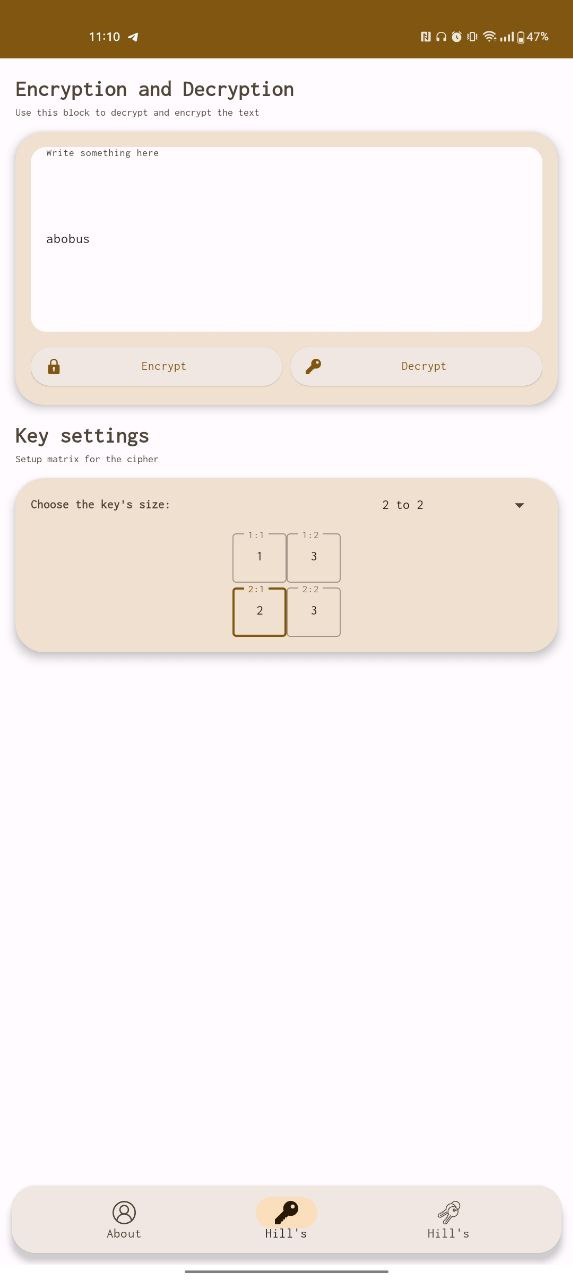
\includegraphics[width=\textwidth]{02_0001}
        \caption{Вводим исходный текст}
    \end{minipage}
    \hfill
    \begin{minipage}{0.3\textwidth}
        \centering
        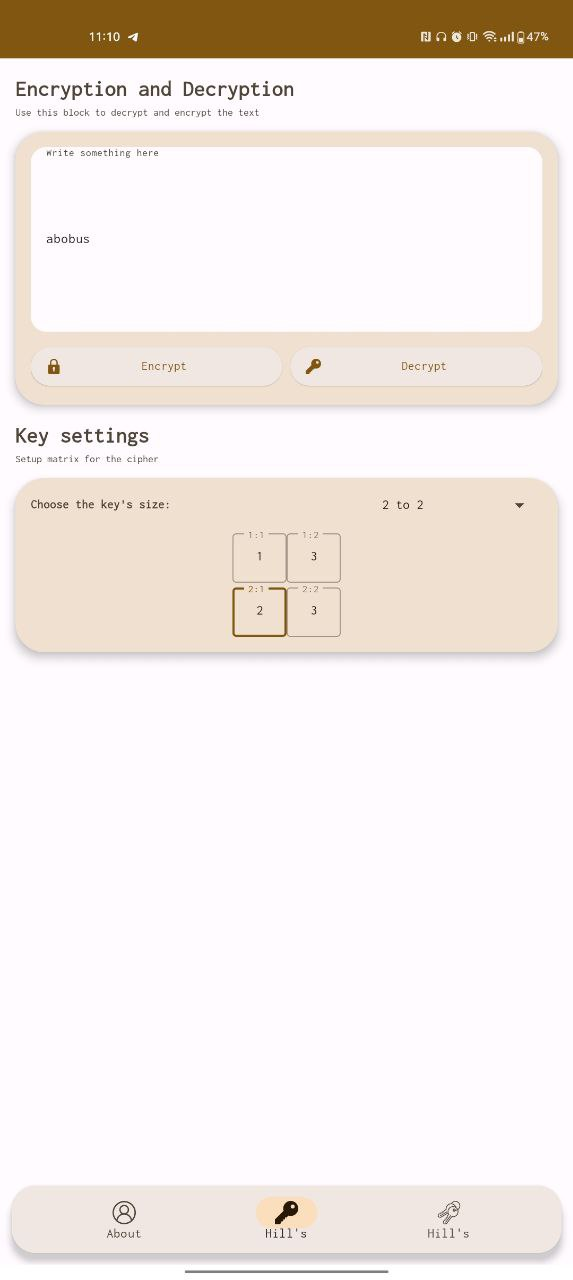
\includegraphics[width=\textwidth]{02_0002}
        \caption{Результат зашифрования}
    \end{minipage}
    \hfill
    \begin{minipage}{0.3\textwidth}
        \centering
        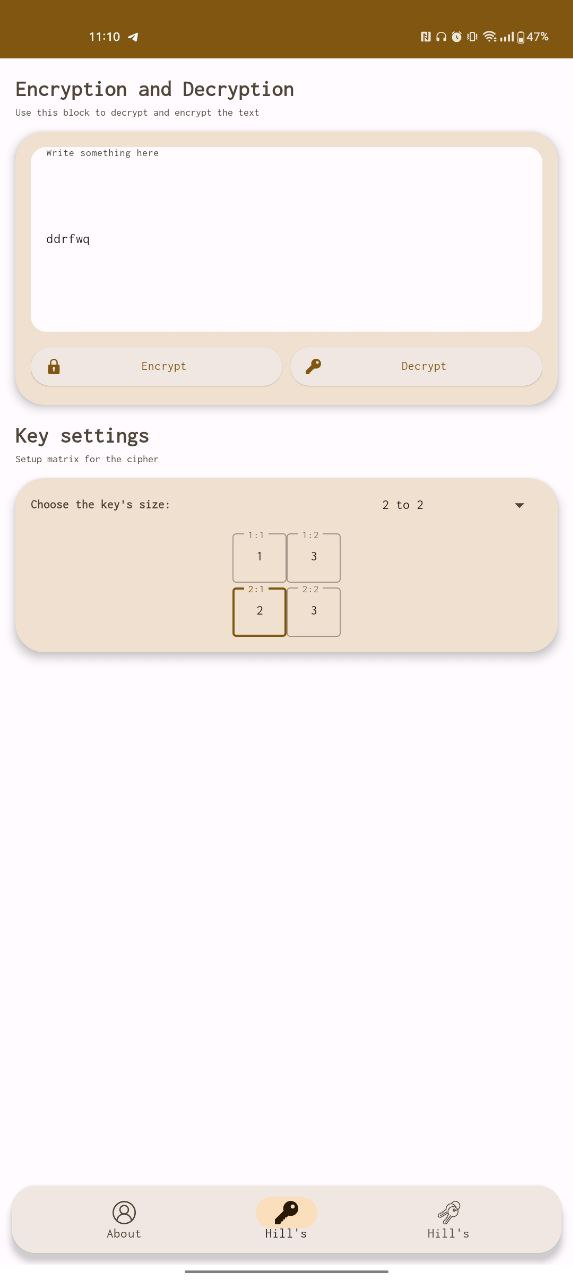
\includegraphics[width=\textwidth]{02_0003}
        \caption{Результат расшифрования}
    \end{minipage}
  \end{figure}

  \subsection{Рекуррентный шифр Хилла}

  \begin{figure}[H]
    \begin{minipage}{0.3\textwidth}
        \centering
        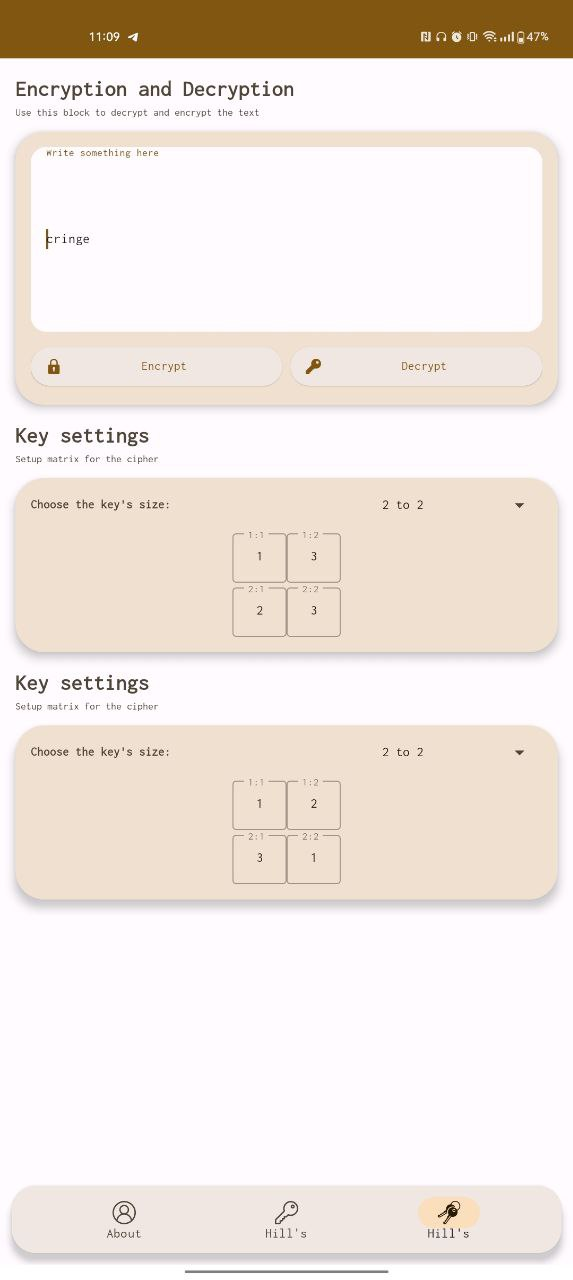
\includegraphics[width=\textwidth]{02_0004}
        \caption{Вводим исходный текст}
    \end{minipage}
    \hfill
    \begin{minipage}{0.3\textwidth}
        \centering
        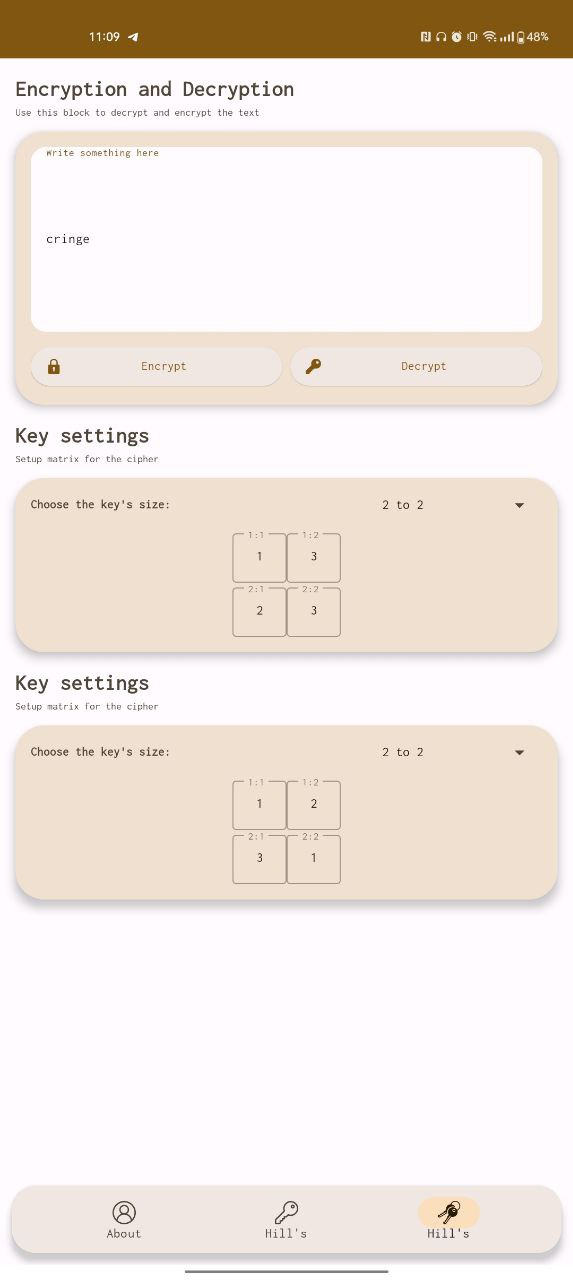
\includegraphics[width=\textwidth]{02_0005}
        \caption{Результат зашифрования}
    \end{minipage}
    \hfill
    \begin{minipage}{0.3\textwidth}
        \centering
        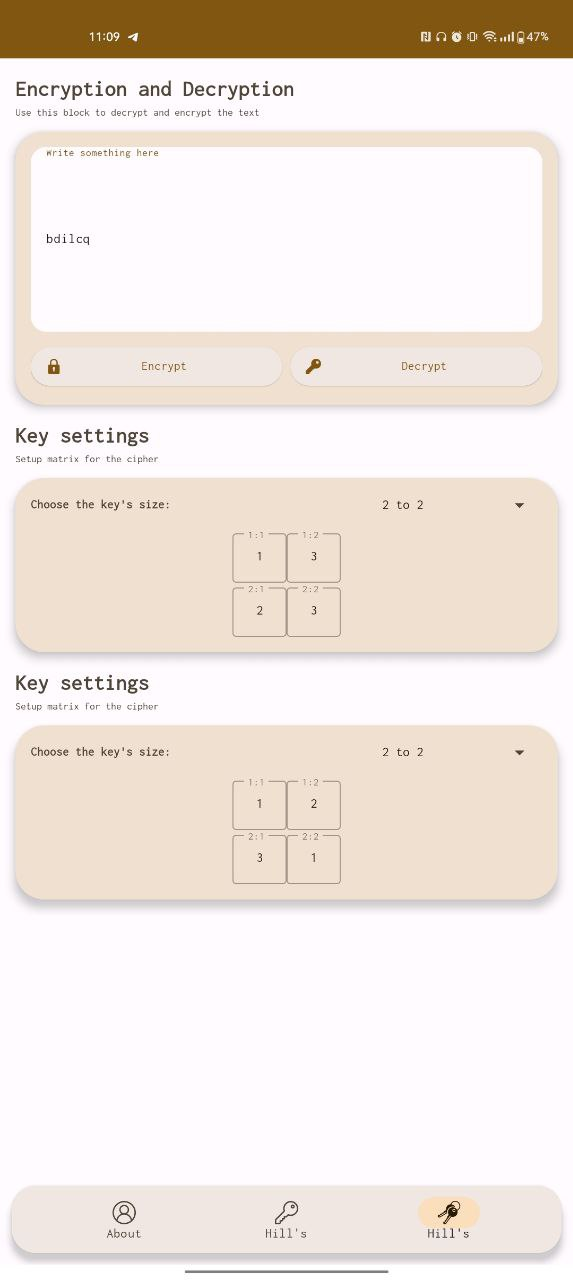
\includegraphics[width=\textwidth]{02_0006}
        \caption{Результат расшифрования}
    \end{minipage}
  \end{figure}

  \newpage
  \section{Криптоанализ}

  В данном разделе я рассматриваю только атаку на основе открытого текста, так 
  как полный перебор потенциально может потребовать слишком много времени, а
  частотный анализ все же имеет достаточно низкую эффективность перед данными
  шифрами.

  Также рассматривается только обычный шифр Хилла, так как в рекуррентном требуется
  лишь составить большую систему - общий вид каждого последующего ключа.

  Допустим, имеется зашифрованная последовательность <<gs nayk ks akxpyw>> и известно,
  что зашифрование производилось ключом размером $2 \times 2$ и что слову <<nayk>> соответсвует
  кусок открытого текста с содержанием <<name>>.

  Выполним приведение буквенных последовательностей к числовым:
  <<nayk>> $ = (13, 0, 24, 10)$, <<name>> $= (13, 0, 12, 4)$. Допустим, что ключ имеет вид:
  \begin{equation}
    K = \begin{pmatrix}
        a & b \\ c & d
    \end{pmatrix}
  \end{equation}

  Тогда исходя из определения операции зашифрования верно:
  \begin{align}
    \begin{pmatrix}
        a & b \\ c & d
    \end{pmatrix} \cdot \begin{pmatrix}
        13 \\ 0
    \end{pmatrix} \mod{26} = \begin{pmatrix}
        13 \\ 0
    \end{pmatrix} &&
    \begin{pmatrix}
        a & b \\ c & d
    \end{pmatrix} \cdot \begin{pmatrix}
        12 \\ 4
    \end{pmatrix} \mod{26}= \begin{pmatrix}
        24 \\ 10
    \end{pmatrix}
  \end{align}

  Эти матричные уравнения можно привести к следующей системе:
  \begin{equation}
    \begin{cases}
        (13\cdot a + 0\cdot b)\mod{26} = 13 \\
        (13\cdot c + 0\cdot d) \mod{26}= 0 \\
        (12\cdot a + 4\cdot b)\mod{26} = 24 \\
        (12\cdot c + 4\cdot d)\mod{26} = 10
    \end{cases} \Leftrightarrow \begin{cases}
        a = 1 \\
        b = 3 \\
        c = 2 \\
        d = 3
    \end{cases}
  \end{equation}

  Получается, что исходный ключ соответсвует:
  \begin{equation}
    K = \begin{pmatrix}
        1 & 3 \\ 2 & 3
    \end{pmatrix}
  \end{equation}

  Если с его помощью расшифровать шифртекст, то получится <<My name is Kostya>>

  \newpage
  \section{Вывод}

  В ходе данной работы были реализованы и протестированы следующие блочные шифры -
  шифр Хилла и Рекуррентный шифр Хилла.

  Оба данных шифра при правильном подборе параметров ключа весьма устойчивы к атакам,
  использующим метод грубой силы, весьма устойчивы также и к частотному анализу.

  Однако атаки на основе открытого текста могут оказаться весьма эффективными.

\end{document}
